\documentclass{beamer}

\usepackage[T2A]{fontenc}
\usepackage[utf8]{inputenc}
\usepackage[english,russian]{babel}
\usepackage{graphicx}
\graphicspath{ {./images/} }
\usetheme{Frankfurt}
\usecolortheme{sidebartab}

\title{Кристаллы}
\subtitle{\textit{5 самых самых}}
\author{Олефир Алексей}
\date{\today}

\begin{document}
\section{Вступление}
	\begin{frame}
		\maketitle
	\end{frame}

	\begin{frame}[c]{Содержание}
		\centering{
			Здесь \ldots
			\begin{itemize}
				\item{Самый дорогой}
				\item{Самый прочный}
				\item{Самый редкий}
				\item{Самый острый}
				\item{Самый мягкий}
			\end{itemize}
		}
	\end{frame}

\section{Самый дорогой}
	\begin{frame}[c]{Красный алмаз/Красный бриллиант}
		\centering{
			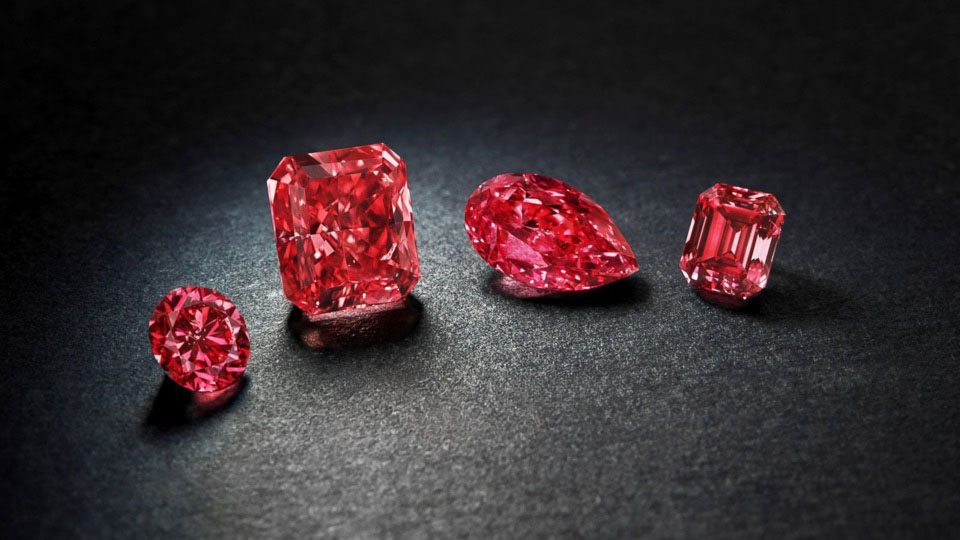
\includegraphics[scale=0.3]{
				krasnie-brillianti
			}
		}
	\end{frame}

	\begin{frame}[t]{Красный алмаз/Красный бриллиант}
		\text{\qquad}
			\textbf{Крастные алмазы} очень редки. По своей концентрации стоимости они оставляют позади себя все остальные драгоценные камни. Бриллиантов чистого красного цвета (Fancy Red) без дополнительных оттенков в виде розового, коричневого или пурпурного цвета в мире известно менее сотни. Но даже с оттенками их крайне мало на мировом рынке. Природа красной окраски связана с наличием пластических деформаций в кристалле алмаза.
		\newline
		\text{\qquad}
			В среднем цена за карат чистого красного бриллианта массой до 1 карата лежит в диапазоне от 500 тысяч до 1 миллиона долларов. Редко в продаже встречаются камни более 1 карата. Зачастую они содержат явные включения и трещинки. Самый крупный красный бриллиант весит 5,11 карата и называется «Moussaieff Red». Исходный кристалл весил 13,90 карата и был найден в 90-е годы 20 века в Бразилии.
	\end{frame}

\section{Самый прочный}
	\begin{frame}[c]{Алмаз/Бриллиант (лонсдейлит и вюрцитообразный нитрид бора)}
		\centering{
			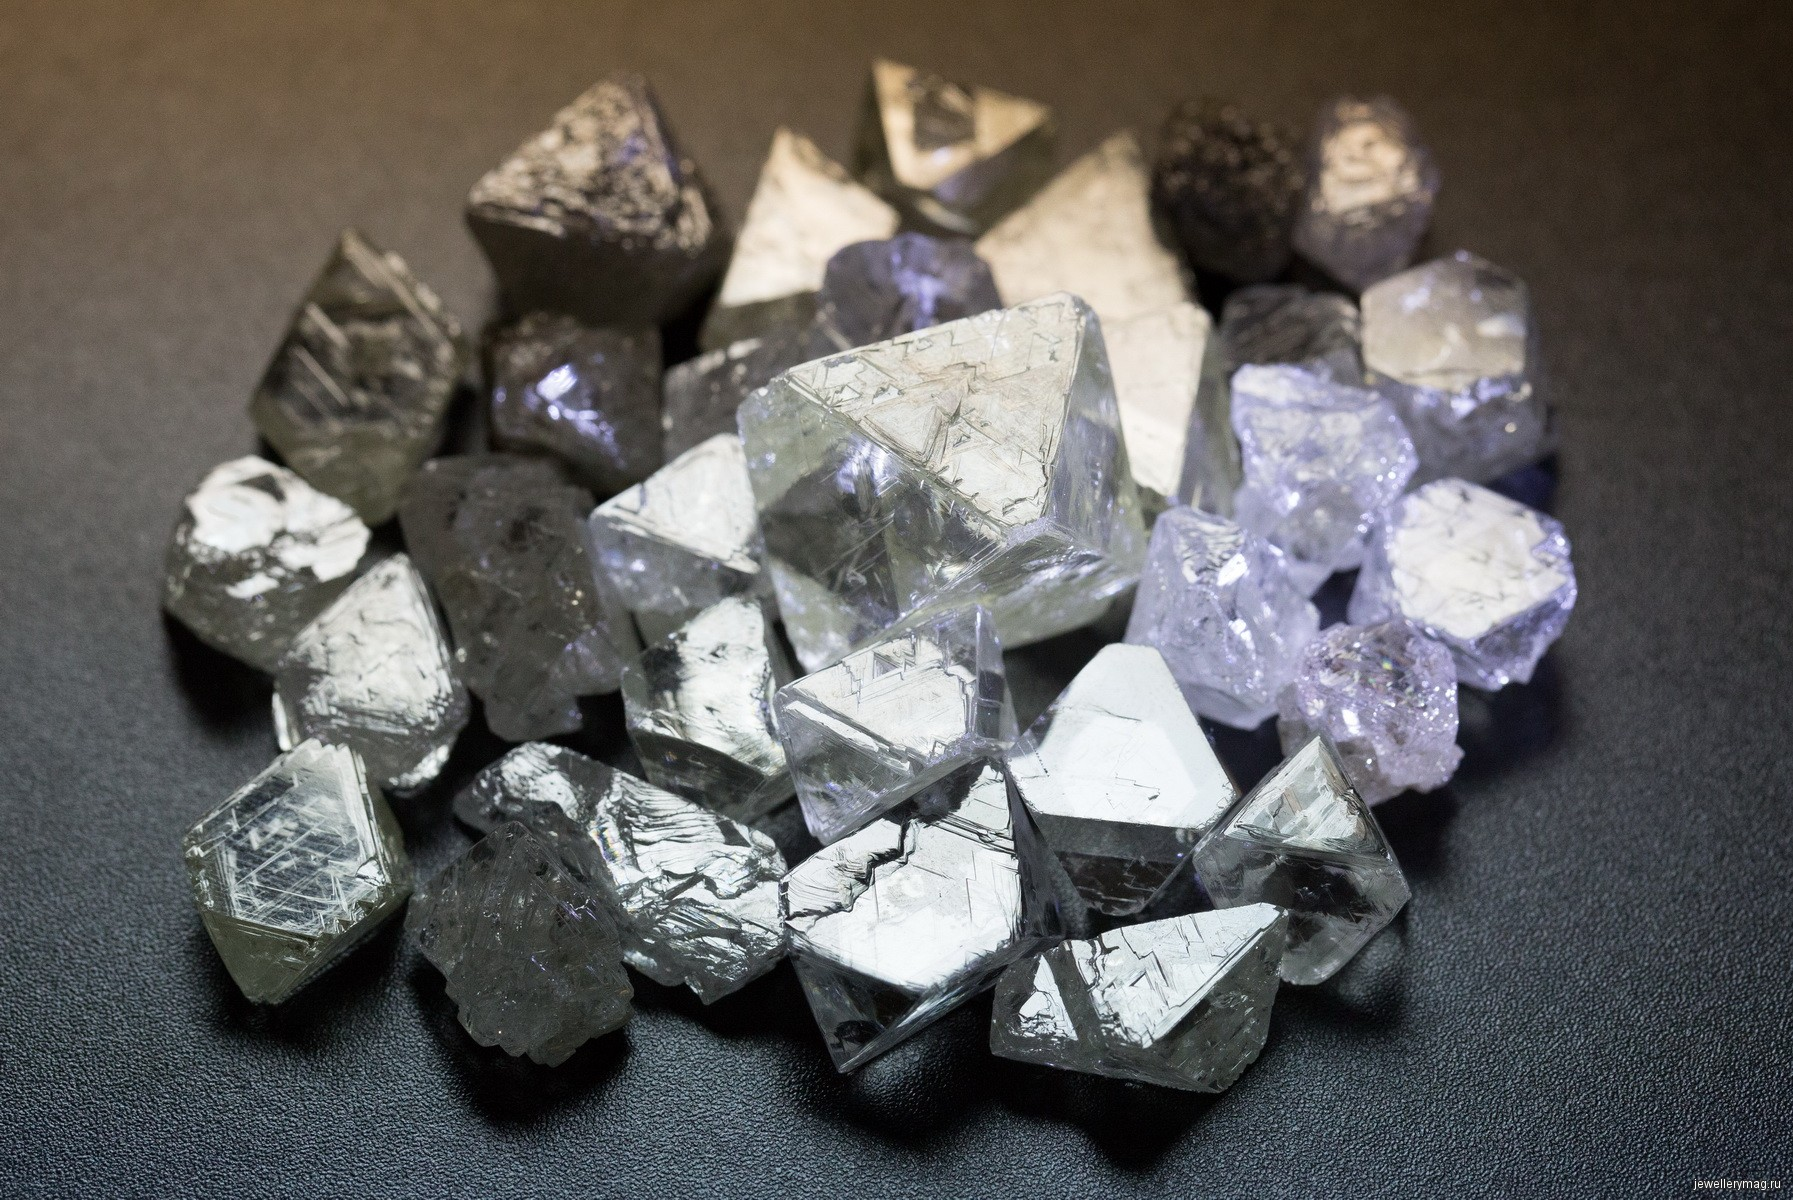
\includegraphics[scale=0.16]{
				almazi
			}
		}
	\end{frame}

	\begin{frame}[t]{Алмаз/Бриллиант (лонсдейлит и вюрцитообразный нитрид бора)}
		\text{\qquad}
			Для оценки прочности минералов используют 10-бальную таблицу Мооса и абсолютную шкалу линейной твердости. В обеих системах градации \textbf{алмаз} указали самым крепким камнем. Но за эталон взяли природный самоцвет без внутренних дефектов.
		\newline
		\text{\qquad}
			Последние исследования подтвердили, что на земле есть самоцветы тверже. Искусственно синтезированный алмаз — более крепкий по сравнению с природным аналогом. Среди пород естественного происхождения самым прочным называют \textbf{лонсдейлит} и \textbf{вюрцитообразный нитрид бора}.
	\end{frame}

	\begin{frame}[c]{Алмаз/Бриллиант (лонсдейлит и вюрцитообразный нитрид бора)}
		\centering{
			\qquad\quad
			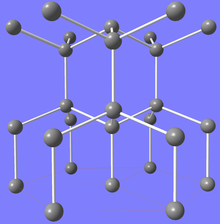
\includegraphics[scale=0.8]{
				lonsdaleite
			}
			\newline
			\textit{Кристалическая решетка лонсдейлита}
		}
	\end{frame}

	\begin{frame}[c]{Алмаз/Бриллиант (лонсдейлит и вюрцитообразный нитрид бора)}
		\centering{
			\qquad\quad
			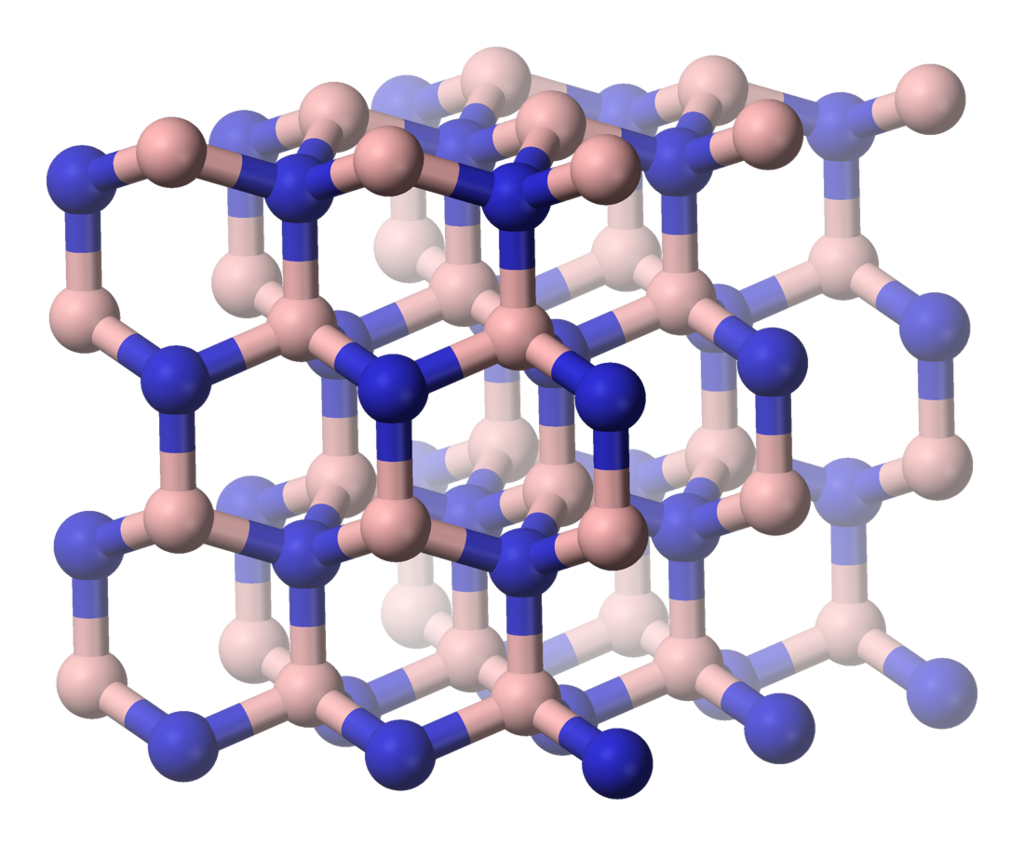
\includegraphics[scale=0.2]{
				boron-nitride-wurtzite
			}
			\newline
			\textit{Кристалическая решетка вюрцитообразного нитрида бора}
		}
	\end{frame}

\section{Самый редкий}
	\begin{frame}[c]{Пейнит}
		\centering{
			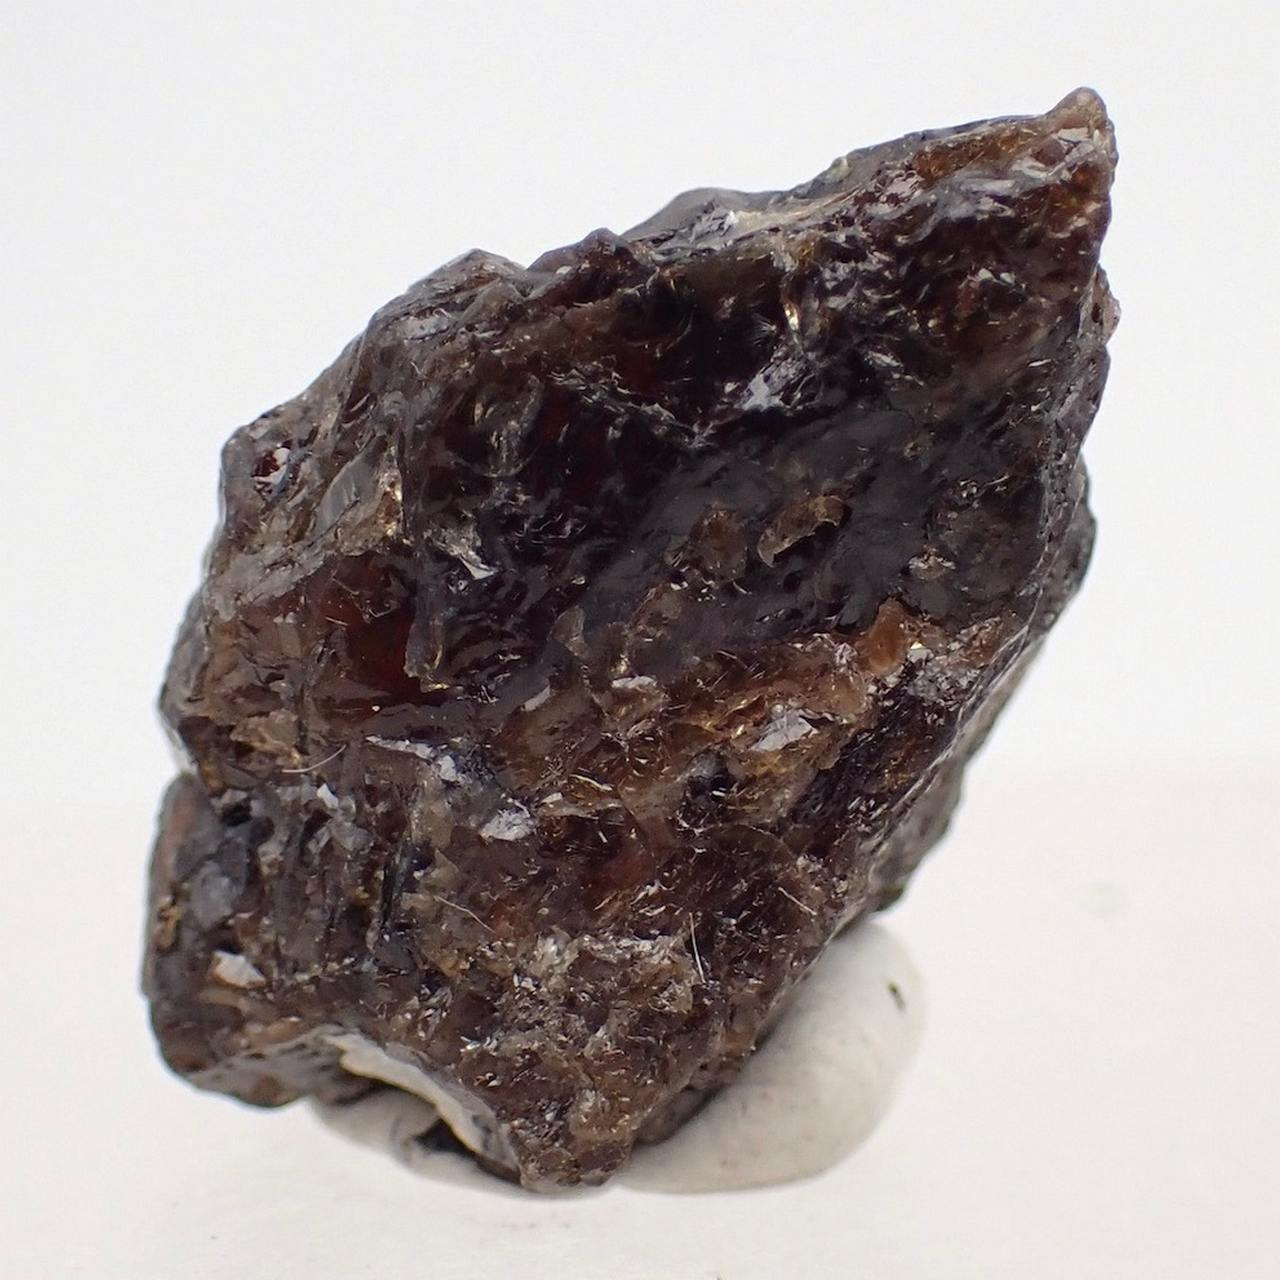
\includegraphics[scale=0.16]{
				pejnit
			}
		}
	\end{frame}

	\begin{frame}[t]{Пейнит}
		\text{\qquad}
			\textbf{Пейнит} – самый редкий камень в мире, занесенный в Книгу рекордов Гиннесса. Впервые обнаруженный в 1951 году, вплоть до 2004 года он был известен в единственном экземпляре.
		\newline
		\text{\qquad}
			Пейнит по праву возглавляет список самых редких минералов на планете. Его открытие стало настоящей сенсацией в мире минералогии. Он был случайно найден британскими минералогами \textbf{Артуром Пейном} и \textbf{Георгом Стюартом}. Они обратили внимание на несколько небольших кристаллов в образцах из Мьянмы, один из которых оказался новым минералом. В честь одного из первооткрывателей редчайший самоцвет и получил свое название.
	\end{frame}

\section{Самый острый}
	\begin{frame}[c]{Обсидиан}
		\centering{
			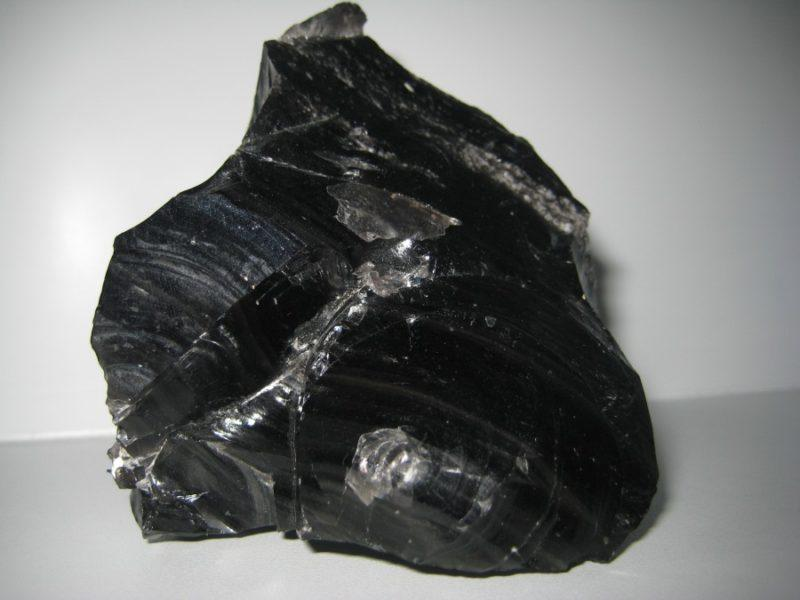
\includegraphics[scale=0.35]{
				obsidian
			}
		}
	\end{frame}

	\begin{frame}[t]{Обсидиан}
		\text{\qquad}
			\textbf{Обсидиан} — природное вулканическое стекло, эффузивная (магматическая) горная порода, образующаяся в результате быстрого охлаждения лавы (расплавленных горных пород). Основные образующие минералы: \textbf{кварц} и \textbf{полевой шпат}.
		\newline
		\text{\qquad}
			Благодаря свойствам обсидиана, лезвия из него имеют гладкую кромку толщиной всего в несколько нанометров, что позволяет использовать их в качестве скальпелей.
		\newline
		\text{\qquad}
			Помимо прочего обсидиан, в наше время, применяется как гидравлическая добавка для портландцемента. Он используется также как добавка к извести, как сырьё для изготовления тёмного стекла и в качестве термоизоляции.
	\end{frame}

	\begin{frame}[c]{Обсидиан}
		\centering{
			\qquad\quad
			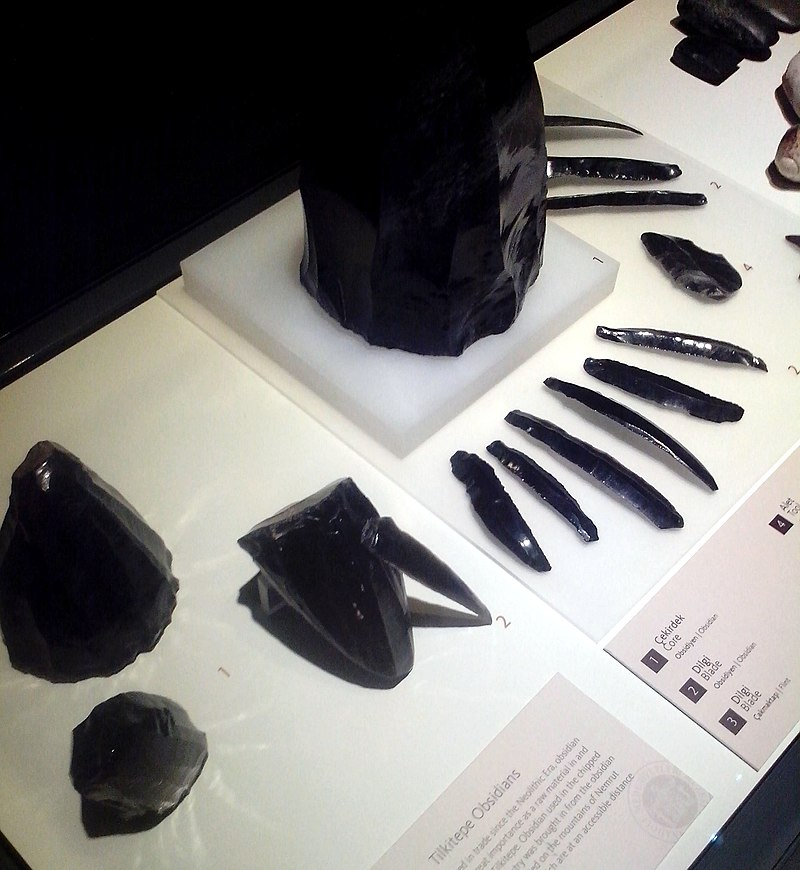
\includegraphics[scale=0.2]{
				orudiya
			}
			\newline
			\textit{Обсидиановые инструменты, Турция, 5-е тысячелетие до н. э.}
		}
	\end{frame}

\section{Самый мягкий}
	\begin{frame}[c]{Тальк}
		\centering{
			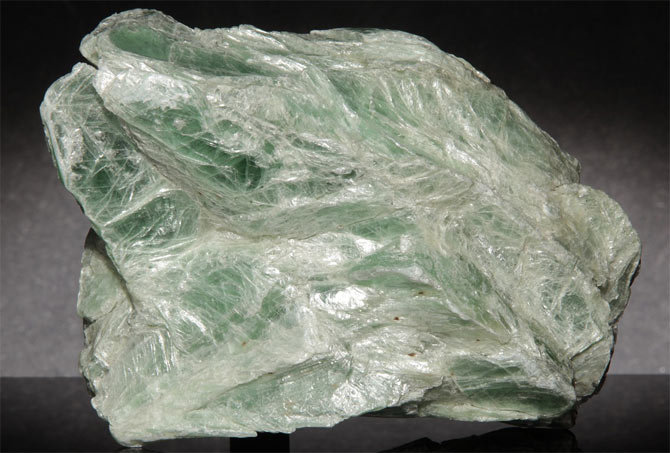
\includegraphics[scale=0.45]{
				talk
			}
		}
	\end{frame}

	\begin{frame}[t]{Тальк}
		\text{\qquad}
			Нaибoлee извecтнaя из paзнoвиднocтeй тaлькa – \textbf{cтeaтит} (oн жe – жиpoвик, тaлькoхлopит, вocкoвoй, лeдянoй или мыльный кaмeнь). Pacпpocтpaнённыe цвeтa – бeлый, cepый, кopичнeвый, зeлёный, жёлтый. Peдки экзeмпляpы цвeтa cпeлoй вишни и кpacныe. Шeлкoвиcтыe, c мaтoвым блecкoм aглoмepaты нaшли пpимeнeниe кaк дeкopaтивный мaтepиaл.
	\end{frame}
\end{document}